\index{general}{Lyapunov Time}
\begin{flushright} {\tiny {\color{gray} mixing\_stirring.tex}} \end{flushright}

Many approaches are taken in the literature when it comes 
to studying mixing/stirring in fluids, and in our case the mantle.

For example, \textcite{sato12} (2012) 
measure the convective stirring efficiency using two Lagrangian methods: 
the first determines the mixing time associated with
different wavelengths of heterogeneity following the approach of \textcite{feri01} (2001)
The second determines the value of
the maximum Finite Time Lyapunov Exponents (FTLE) as described in 
\textcite{fasa03} (2003), and measures the rate at
which heterogeneities are stretched by mantle motions.

In the review of \textcite{vavt24} by Nicolas Coltice, his review reads:
\begin{displayquote}
{\color{darkgray}
``
The first studies of mantle mixing date back to the 1980’s and one of the 
difficulty was to deal with scales. So 2 approaches were taken: one dealing explicitly 
with scales, such as the authors do here with configurational entropy. It was in 
relationship with the observations of heterogeneities at all scales (marble cake like at 
first, more comprehensive nowadays with mid-ocean ridge heterogeneities etc…). 
The other approach is to work with the theory of dynamic systems, because mantle convection 
is chaotic. The use of Lyapunov exponent characterize the local and global properties of 
stretching of heterogeneities. Mixing happens when an heterogeneity is stretched at a 
scale at which chemical diffusion operates. This scale for the Earth is about 1cm I 
would say (some papers talk about it). Lyapunov exponent are a form of stretching rate 
when mixing is chaotic. Configurational entropy and Lyapunov exponent can be related 
with Ergodicity theory. 
''
}
\end{displayquote}





In \textcite{taxi02} (2002) we read: 

\begin{displayquote}
{\color{darkgray}
``
Two-dimensional simulations of simple mantle convection (\textcite{chri89}, 1989; 
\textcite{ketu90}, 1990; \textcite{scha94}) suggest that for whole-mantle 
convection the mantle should be homogenized in a time-scale of less than 1 Gyr, although
unmixed islands may remain. Non-Newtonian rheology, which is thought to be 
important in the upper mantle \cite{kawu93}, may somewhat inhibit mixing (\textcite{tepy98}, 1998). 
The rate at which blobs of anomalous (e.g. primitive) material are stretched
and assimilated into the flow depends on their relative viscosity; very viscous blobs
can survive intact for many mantle overturns (\textcite{mang96}, 1996).
\\
In three-dimensional geometry with only poloidal flow, mixing may be significantly
less efficient than in two dimensions (\textcite{schh95}, 1995; \textcite{schh96}, 1996) 
but, if the toroidal flow associated with plate motions is 
included (\textcite{gaot91}, 1991), mixing can instead be more efficient 
(\textcite{feri98} (1998)).
\\
High viscosity in the deep mantle is not sufficient to maintain different reservoirs
over geological time-scales (\textcite{feri01}, 2001; van Keken \& Ballentine 1998,
1999), in contrast to predictions from earlier calculations at lower convective vigour
(\textcite{guda86b}, 1986). Part of the reason for this apparent discrepancy is that
the latter study used a kinematically driven flow rather than buoyancy-driven flow.
Since a viscosity jump does not affect densities, thermal buoyancy-driven flow has no
problem crossing it, so substantial mass exchange occurs between upper and lower
mantles. Buoyancy is thus necessary to maintain separate reservoirs.
''
}
\end{displayquote}


In \textcite{gowh06} (2006) we find
\begin{displayquote}
{\color{darkgray}
``
Heterogeneities in a convecting fluid are deformed by
stirring and finally erased by diffusive mixing. Chemical diffusion in mantle rock
acts on the scale of centimetres over the lifetime of the Earth, but our models
resolve km-scales. Therefore this paper deals only with convective stirring. Some
nice studies about mantle stirring and mixing in 2-d have been done (e.g. 
\cite{chri89,guda86b,kest91,ketu90,mebo95,olyb84,olyb84b,teyl96,teyp97,tepy98}).
Unfortunately, results from studies in 2-d can be extrapolated to 3-d only in a limited
manner. Tracers in 3-d poloidal stationary convection move on 2-d toruslike
surfaces. Stirring is constrained to these surfaces. Cross-cell stirring becomes possible
in time-dependent flows, but may not be very efficient \cite{schh96}. Large-scale stirring is
enhanced by a toroidal component, but convectively isolated islands of laminar
stirring may remain \cite{feri98}. Convection in the Earth is time-dependent and the surface
planform shows a strong toroidal component today. Since there is currently no
general understanding about the stirring behaviour of the mantle, a case-by-case
study of different models is necessary.
''
}
\end{displayquote}


\textcite{kest91} (1991) looked into chaotic mixing and state:
\begin{displayquote}
{\color{darkgray}
``
The extent of mixing is quantitatively measured by 
calculating the deformation undergone by passive, elliptical
strain markers. Deformation of a marker is characterized by
its elongation $a/a_0$, where $a$ is the length of the semimajor
axis and $a_0$, is the initial length. For infinitesimal markers,
deformation is controlled by the local flow field and is 
obtained by integrating the strain rate tensor along the particle's 
trajectory \cite{ketu90}. The aspect ratio $\epsilon$ and orientation $\theta$ 
of the ellipse vary with the nondimensional time according to
\begin{equation}
\frac{d\epsilon}{dt}=2 \epsilon (\bar{\alpha} \cos 2\theta + \bar{\beta} \sin 2\theta)
\label{eq:mixx1}
\end{equation}
and
\begin{equation}
\frac{d\theta}{dt}=\left(\frac{\epsilon^2 +1}{\epsilon^2-1} \right)
(-\bar{\alpha} \sin 2\theta + \bar{\beta} \cos 2\theta) + \bar{\omega}.
\label{eq:mixx2}
\end{equation}
The components of the nondimensional strain tensor $\bar{\alpha}$,
$\bar{\beta}$ and $\bar{\omega}$ are defined by
\begin{eqnarray}
\bar{\alpha} &=& \frac{\partial u}{\partial x} \\
\bar{\beta}  &=& \frac12\left( \frac{\partial u}{\partial y}+\frac{\partial v}{\partial x}\right)\\
\bar{\omega} &=& \frac12\left( \frac{\partial u}{\partial y}-\frac{\partial v}{\partial x}\right)
\end{eqnarray}
These equations define the evolution of an infinites`imal
strain marker in an arbitrary, two-dimensional flow. Given
the path of a particle in any flow, we can evaluatei
$\bar{\alpha}$, $\bar{\beta}$ and $\bar{\omega}$
at each position of the particle, and integrate \eqref{eq:mixx1} and \eqref{eq:mixx2}
along the particle path to obtain the deformation history of a
strain marker.
These equations are derived in \textcite{kell93} (1993).
''
}
\end{displayquote}

In \textcite{fasa03} we find this important distinction:
\begin{displayquote}
{\color{darkgray}
``
Stirring involves the repeated action of stretching 
and folding of a fluid element, while mixing
also involves diffusion at small scales. The
term stirring is more appropriate for the mantle,
since rocks chemical diffusivity is only $10^{-15}-10^{-20}$.
''
}
\end{displayquote}



In \textcite{saad11} (2011) we find:
\begin{displayquote}
{\color{darkgray}
``
We measure the convective stirring efficiency using
two Lagrangian methods: \\
the first determines the mixing
time associated with different wavelengths of heterogeneity
following the approach of \textcite{feri01} (2001).\\
The second determines the value of the maximum Finite Time
Lyapunov Exponents (FTLE), $\lambda^+$ as described by 
\textcite{fasa03} (2003), and measures the rate at which 
heterogeneities will be stretched by mantle motions. These methods
were applied after each experiment had reached statistical
steady state.
''
}
\end{displayquote}


\textcite{colt05} (2005) looked at 
convective mixing in degassing the Earth's mantle
and describes his methodology as follows:
\begin{displayquote}
{\color{darkgray}
``
To follow stretching and mimic the chemical
evolution of the system, passive particles are tracked
into the flow. Their position x into the convection box
evolves according to
\[
\frac{\partial x}{\partial t} = u(x,t),
\]
$u$ being the local velocity. To solve this equation, a
time integration method and an interpolation of the
velocity between grid nodes are needed. For sake of
consistency, the velocity of a particle lying between
grid nodes is naturally interpolated with the bilinear
shape functions of the finite element formulation in
ConMan. A fifth-order Runge–Kutta scheme is
used for the time integration. In the simulations, I
have checked that the number of particles is always
statistically sufficient (increasing this number does
not change the results).

Two simple models can describe the two end-
members of mixing dynamics: regular (or laminar)
and chaotic (or turbulent) mixing \cite{olyb84b}. Regular
mixing occurs in 2D steady-state flows where the
trajectories of particles are identical to streamlines. In
this regime, an initial distance $l_0$ between two
particles is stretched into a new distance $l$ that
increases linearly with time and proportionally to the
strain rate. The stretching of a distance is parameterized by
\[
\epsilon= l/l_0
\]
which depends linearly on the time as
\begin{equation}\label{eq:mixx:05}
\epsilon(t) = 1+\dot \varepsilon t
\end{equation}
where $\dot{\varepsilon}$ is the Lagrangian strain rate. 
The Lagrangian strain rate is the strain rate experienced locally
by the line as it is moving into the flow. In the
calculations, the Lagrangian strain rate is always
lower than the Eulerian strain rate which is the
second invariant of the local strain rate tensor.

Chaotic mixing occurs when the dimensionality of
the system is larger and where particle trajectories get
more complex. In 2D, time-dependent systems show
this behavior and two particles can follow completely
different path-lines though they were infinitely close
initially. In 3D, even steady flows can produce chaotic
Lagrangian mixing, enhanced by the presence of a
toroidal component \cite{feri98}. Stretching in such a flow
evolves exponentially with time
\[
\epsilon (t) = \exp (\dot \varepsilon t)
\]
The simplicity of these models is that they only
depend on one parameter, the Lagrangian strain rate $\dot\varepsilon$.
This parameter is chosen to be the quantitative
measurement of average mixing in the numerical
experiments. 


\begin{center}
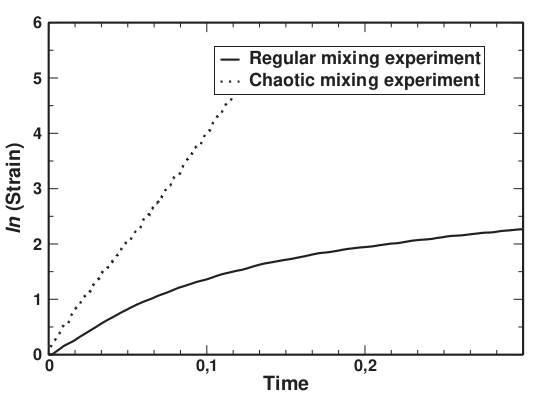
\includegraphics[width=6cm]{images/mixing/colt05}\\
Strain as a function of time in two convection simulations
illustrating regular mixing (internal heating, Ra i = 106) and chaotic
mixing (basal heating, Ra b = 105).
\end{center}


As illustrated by the figure above, the numerical
experiments display strain evolutions that can be well
explained by one of the two end-members of mixing
dynamics

To compute the local stretching $\epsilon$ around a particle,
I follow the distance between two initially very close
particles. The larger the distance, the larger the error
on the local stretching. Hence, this distance has to be
renormalized along the direction of stretching at every
time step \cite{feri98}. At a time $t$, the estimate of the
Lagrangian strain rate is
\[
\dot\varepsilon = \frac{\log (\epsilon)}{t}
\]
The bulk Lagrangian strain rate is the average over
all the couples of particles (20,000 were sufficient). In
regular mixing flows, the computed ė would be much
lower than the theoretical $\dot{\varepsilon}$ of Eq.~
\eqref{eq:mixx:05}.
''
}
\end{displayquote}



\textcite{cosc06} (2006)
show that mixing in 3-D time-dependent convection is as efficient as
in 2-D, and only depends on convective vigor.
compute mixing times of thermal and chemical heterogeneities in
the early Earth of 10 and 100 Myrs respectively.
They write:
\begin{displayquote}
{\color{darkgray}
``
To compute the Lagrangian strain rates, we follow the
distance d(t) between particle twins advected in the flow
using a 4th-order Runge-Kutta scheme. The Lagrangian
strain rate, i.e. finite-time Lyapunov exponent, is computed
assuming that for each couple of tracers, stretching $d(t)/d(0)$
occurs as
\[
\frac{d(t)}{d(0)} = \exp ( \dot\varepsilon t)
\]
Averaging $\dot{\varepsilon}$ over the tracer couples gives the bulk
Lagrangian strain rate characterizing the stretching ability
of the flow \cite{colt05}. If the computed bulk
Lagrangian strain rate tends toward 0, mixing is regular,
otherwise it is chaotic. To start the experiment, the
distribution of the couples of tracers is homogeneous
throughout the box. In the 3-D calculations, up to
10,000,000 tracers are used for an accurate description of
the Lagrangian strain-rate field in 3-D.
''
}
\end{displayquote}

Based on these, we need to look at the Lyapunov exponent (and the 
Finite Time Lyapunov Exponent, i.e. FTLE).

%---------------------------------
\subsection{The Lyapunov exponent}

%from wiki

Simply put, the Lyapunov time is the characteristic timescale on which a dynamical system is chaotic.
 It is defined as the inverse of a system's largest Lyapunov exponent.

The Lyapunov time mirrors the limits of the predictability of the system. By convention, it is defined 
as the time for the distance between nearby trajectories of the system to increase by a factor of $e$. 
However, measures in terms of 2-foldings and 10-foldings are sometimes found, since they correspond to 
the loss of one bit of information or one digit of precision respectively.

The Lyapunov exponent or Lyapunov characteristic exponent of a dynamical system is a quantity 
that characterizes the rate of separation of infinitesimally close trajectories. 
Quantitatively, two trajectories in phase space with initial separation $\delta \mathbf{Z}_0$ 
diverge (provided that the divergence can be treated within the linearized approximation) at a rate given by
\[
|\delta \mathbf{Z} (t)|\approx e^{\lambda t}|\delta \mathbf {Z} _{0}| 
\]
where $\lambda$ is the Lyapunov exponent. 

Measuring the Lyapunov exponent or time (or related quantities) is relevant in the context of mantle stirring. 
On the one hand it is argued that the mantle is convecting and very efficient at mixing resulting in a 
somewhat homogenous composition. On the other hand, there is are modeling studies that suggest that
whole-mantle convection can preserve heterogeneity in the presence of well-mixed mantle. 

%from vazh99
Mixing takes place by the repeated stretching
and folding of interfaces. A measure of the
mixing efficiency is the time evolution of the area of
the mixing surface. Maximum efficiency of mixing
is reached with turbulent mixing behavior where
One can formally show whether mixing is laminar or turbulent by evaluating the Luyaponov exponents $\sigma$ .
These are of the form:
\[
\sigma = \lim_{t\rightarrow \infty} \lim_{X\rightarrow 0} \left[  \frac{1}{t} \ln \left( \frac{X(t)}{X(t=0)} \right)   \right]
\]
where $X(t)$ is the length of this segment at time t.
Non-zero Luyaponov exponents indicate that
stretching is exponential and the larger the exponent,
the more efficient mixing is.
However, the limits in the above equation are difficult to evaluate and the interpretation 
of the 'finite-time' Luyaponov exponent, where both limits are truncated, is difficult to formalize.


In \textcite{vazh99} (1999) the authors use a steady state velocity
pattern obtained for a model of present-day mantle convection. The velocity model is
based on the solution of the Stokes equations in a 3D spherical model with variable rheology.
To study mixing, they release particles in the velocity model and follow 
these by numerical integration. 

\begin{center}
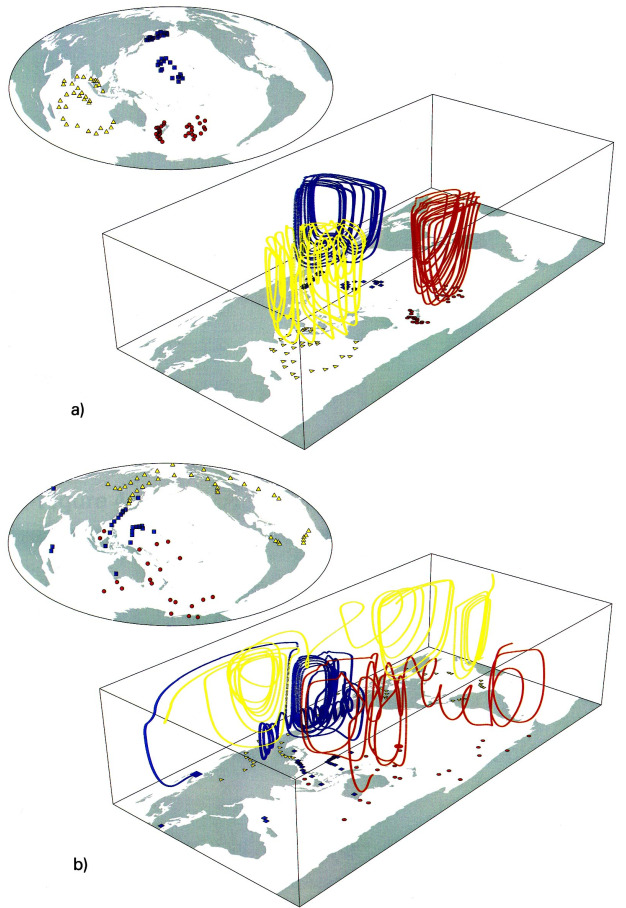
\includegraphics[width=6cm]{images/mixing/vazh99}\\
{\captionfont a) The three particles in this plot were
selected for their relatively regular pattern. 
b) Three other particles that traverse a large portion of the model. These particles feel 
the strong toroidal motion and their paths form corkscrew-like patterns. 
They indicate that certain parts of the model can exhibit strong mixing. 
Taken from \textcite{vazh99} (1999).}
\end{center}

Rather than calculating the exponents explicitly, the authors 
use an approximation to the finite-time,
finite-length Lyaponov exponent by evaluating the distance between two points that are closely spaced
at time $t=0$. For this they compute the advection of a
large number of 10 km long line segments that were
originally at 1500 km depth. The length of these segments is approximated by the distance between the
endpoints and the results are summarized in the following figure:

\begin{center}
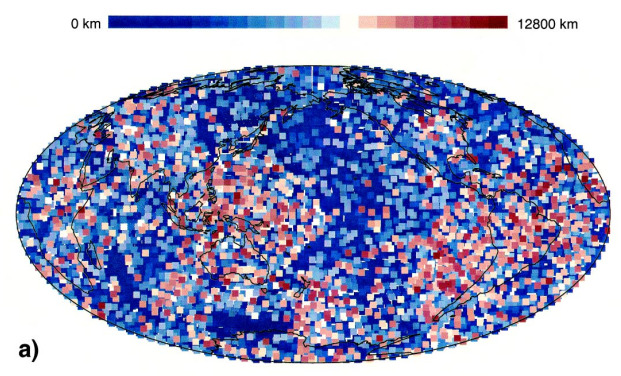
\includegraphics[width=7cm]{images/mixing/vazh99b}\\
{\captionfont Length
of the line segment after 4 billion years. Approximately 14,000 line segments were released with 
regular spacing at 1500 km depth. The length of the segment is indicated by the colored symbols 
that are plotted at the initial position. The results indicate that there is a strong
diversity in mixing behavior. In some regions (north Pacific, parts under the Indian/Australian plate) 
stretching is very limited, indicating laminar and consequently inefficient mixing. Regions that 
are under strong toroidal surface motion (western Pacific, Nazca and South
America) show very efficient stretching of up to the maximum length of the diameter of the Earth. 
Taken from \textcite{vazh99} (1999).}
\end{center}


In \textcite{becr14} (2014) the authors estimate for the first time the limit of predictability of Earth’s
mantle convection. Following the twin experiment method, we compute the Lyapunov time (i.e., e-folding
time) for state of the art 3-D spherical convection models, varying rheology, and Rayleigh number.


Reconstruction of mantle convection and surface tectonics with (ensemble) Kalman filter:
\textcite{bocf16} (2016),
\textcite{bofc18} (2018).

Investigating the initial condition
of mantle models using data assimilation. PhD thesis. \textcite{pric16} (2016).


\Literature

\textcite{pier91} (1991),
\textcite{cobs15} (2015),
\textcite{canl15} (2015),
\textcite{thsf24} (2024).

%-----------------------------------------------
\subsection{Following patches of passively advected markers}

In \textcite{gurn86} (1986) the stirring
of a small, passive
heterogeneity
in an unsteady circulation
is investigated by following
the boundary of the heterogeneity;
the circulation mimics features
of plate-scale flow.
After initial release,
the heterogeneity is stirred
and subsequently consists of at least one
large "blob" connected to long, but thin tendrils.

\begin{center}
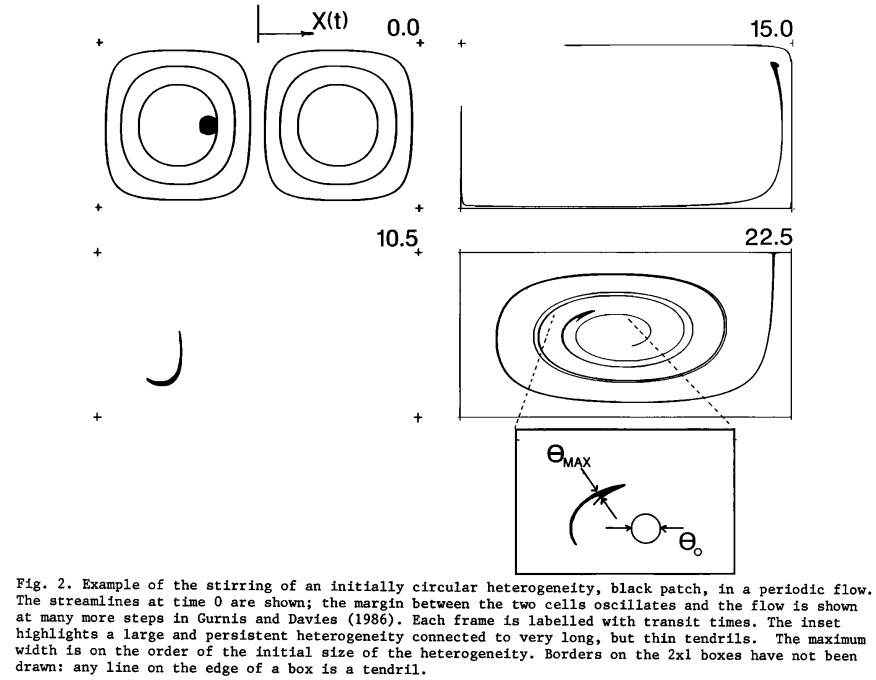
\includegraphics[width=9cm]{images/mixing/gurn86}
\end{center}

%-----------------------------------------------
\subsection{Hyperbolic persistence time method}

This method is presented in \textcite{fasa03} (2003).
Looks complex, and too long to copy paste here.



%-----------------------------------------------
\subsection{configurational 'Shannon' entropy}

\textcite{gobo02} (2002), 
\textcite{cakm06} (2006),
\textcite{nake07} (2007), 
\textcite{pedp15} (2015),
\textcite{bipe18} (2018),
\textcite{vatv24} (2024).



